\documentclass[1p]{elsarticle_modified}
%\bibliographystyle{elsarticle-num}

%\usepackage[colorlinks]{hyperref}
%\usepackage{abbrmath_seonhwa} %\Abb, \Ascr, \Acal ,\Abf, \Afrak
\usepackage{amsfonts}
\usepackage{amssymb}
\usepackage{amsmath}
\usepackage{amsthm}
\usepackage{scalefnt}
\usepackage{amsbsy}
\usepackage{kotex}
\usepackage{caption}
\usepackage{subfig}
\usepackage{color}
\usepackage{graphicx}
\usepackage{xcolor} %% white, black, red, green, blue, cyan, magenta, yellow
\usepackage{float}
\usepackage{setspace}
\usepackage{hyperref}

\usepackage{tikz}
\usetikzlibrary{arrows}

\usepackage{multirow}
\usepackage{array} % fixed length table
\usepackage{hhline}

%%%%%%%%%%%%%%%%%%%%%
\makeatletter
\renewcommand*\env@matrix[1][\arraystretch]{%
	\edef\arraystretch{#1}%
	\hskip -\arraycolsep
	\let\@ifnextchar\new@ifnextchar
	\array{*\c@MaxMatrixCols c}}
\makeatother %https://tex.stackexchange.com/questions/14071/how-can-i-increase-the-line-spacing-in-a-matrix
%%%%%%%%%%%%%%%

\usepackage[normalem]{ulem}

\newcommand{\msout}[1]{\ifmmode\text{\sout{\ensuremath{#1}}}\else\sout{#1}\fi}
%SOURCE: \msout is \stkout macro in https://tex.stackexchange.com/questions/20609/strikeout-in-math-mode

\newcommand{\cancel}[1]{
	\ifmmode
	{\color{red}\msout{#1}}
	\else
	{\color{red}\sout{#1}}
	\fi
}

\newcommand{\add}[1]{
	{\color{blue}\uwave{#1}}
}

\newcommand{\replace}[2]{
	\ifmmode
	{\color{red}\msout{#1}}{\color{blue}\uwave{#2}}
	\else
	{\color{red}\sout{#1}}{\color{blue}\uwave{#2}}
	\fi
}

\newcommand{\Sol}{\mathcal{S}} %segment
\newcommand{\D}{D} %diagram
\newcommand{\A}{\mathcal{A}} %arc


%%%%%%%%%%%%%%%%%%%%%%%%%%%%%5 test

\def\sl{\operatorname{\textup{SL}}(2,\Cbb)}
\def\psl{\operatorname{\textup{PSL}}(2,\Cbb)}
\def\quan{\mkern 1mu \triangleright \mkern 1mu}

\theoremstyle{definition}
\newtheorem{thm}{Theorem}[section]
\newtheorem{prop}[thm]{Proposition}
\newtheorem{lem}[thm]{Lemma}
\newtheorem{ques}[thm]{Question}
\newtheorem{cor}[thm]{Corollary}
\newtheorem{defn}[thm]{Definition}
\newtheorem{exam}[thm]{Example}
\newtheorem{rmk}[thm]{Remark}
\newtheorem{alg}[thm]{Algorithm}

\newcommand{\I}{\sqrt{-1}}
\begin{document}

%\begin{frontmatter}
%
%\title{Boundary parabolic representations of knots up to 8 crossings}
%
%%% Group authors per affiliation:
%\author{Yunhi Cho} 
%\address{Department of Mathematics, University of Seoul, Seoul, Korea}
%\ead{yhcho@uos.ac.kr}
%
%
%\author{Seonhwa Kim} %\fnref{s_kim}}
%\address{Center for Geometry and Physics, Institute for Basic Science, Pohang, 37673, Korea}
%\ead{ryeona17@ibs.re.kr}
%
%\author{Hyuk Kim}
%\address{Department of Mathematical Sciences, Seoul National University, Seoul 08826, Korea}
%\ead{hyukkim@snu.ac.kr}
%
%\author{Seokbeom Yoon}
%\address{Department of Mathematical Sciences, Seoul National University, Seoul, 08826,  Korea}
%\ead{sbyoon15@snu.ac.kr}
%
%\begin{abstract}
%We find all boundary parabolic representation of knots up to 8 crossings.
%
%\end{abstract}
%\begin{keyword}
%    \MSC[2010] 57M25 
%\end{keyword}
%
%\end{frontmatter}

%\linenumbers
%\tableofcontents
%
\newcommand\colored[1]{\textcolor{white}{\rule[-0.35ex]{0.8em}{1.4ex}}\kern-0.8em\color{red} #1}%
%\newcommand\colored[1]{\textcolor{white}{ #1}\kern-2.17ex	\textcolor{white}{ #1}\kern-1.81ex	\textcolor{white}{ #1}\kern-2.15ex\color{red}#1	}

{\Large $\underline{10_{118}~(K10a_{88})}$}

\setlength{\tabcolsep}{10pt}
\renewcommand{\arraystretch}{1.6}
\vspace{1cm}\begin{tabular}{m{100pt}>{\centering\arraybackslash}m{274pt}}
\multirow{5}{120pt}{
	\centering
	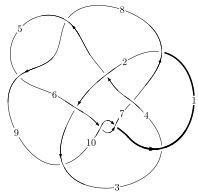
\includegraphics[width=112pt]{../../../GIT/diagram.site/Diagrams/png/202_10_118.png}\\
\ \ \ A knot diagram\footnotemark}&
\allowdisplaybreaks
\textbf{Linearized knot diagam} \\
\cline{2-2}
 &
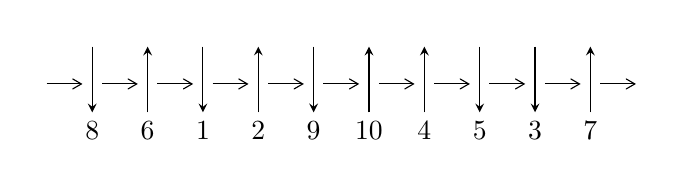
\begin{tikzpicture}[x=20pt, y=17pt]
	% nodes
	\node (C0) at (0, 0) {};
	\node (C1) at (1, 0) {};
	\node (C1U) at (1, +1) {};
	\node (C1D) at (1, -1) {8};

	\node (C2) at (2, 0) {};
	\node (C2U) at (2, +1) {};
	\node (C2D) at (2, -1) {6};

	\node (C3) at (3, 0) {};
	\node (C3U) at (3, +1) {};
	\node (C3D) at (3, -1) {1};

	\node (C4) at (4, 0) {};
	\node (C4U) at (4, +1) {};
	\node (C4D) at (4, -1) {2};

	\node (C5) at (5, 0) {};
	\node (C5U) at (5, +1) {};
	\node (C5D) at (5, -1) {9};

	\node (C6) at (6, 0) {};
	\node (C6U) at (6, +1) {};
	\node (C6D) at (6, -1) {10};

	\node (C7) at (7, 0) {};
	\node (C7U) at (7, +1) {};
	\node (C7D) at (7, -1) {4};

	\node (C8) at (8, 0) {};
	\node (C8U) at (8, +1) {};
	\node (C8D) at (8, -1) {5};

	\node (C9) at (9, 0) {};
	\node (C9U) at (9, +1) {};
	\node (C9D) at (9, -1) {3};

	\node (C10) at (10, 0) {};
	\node (C10U) at (10, +1) {};
	\node (C10D) at (10, -1) {7};
	\node (C11) at (11, 0) {};

	% arrows
	\draw[->,>={angle 60}]
	(C0) edge (C1) (C1) edge (C2) (C2) edge (C3) (C3) edge (C4) (C4) edge (C5) (C5) edge (C6) (C6) edge (C7) (C7) edge (C8) (C8) edge (C9) (C9) edge (C10) (C10) edge (C11) ;	\draw[->,>=stealth]
	(C1U) edge (C1D) (C2D) edge (C2U) (C3U) edge (C3D) (C4D) edge (C4U) (C5U) edge (C5D) (C6D) edge (C6U) (C7D) edge (C7U) (C8U) edge (C8D) (C9U) edge (C9D) (C10D) edge (C10U) ;
	\end{tikzpicture} \\
\hhline{~~} \\& 
\textbf{Solving Sequence} \\ \cline{2-2} 
 &
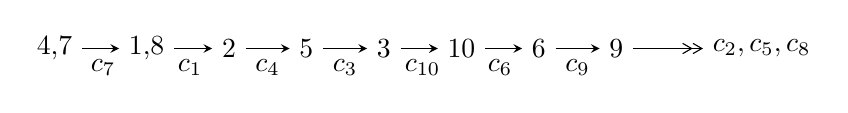
\begin{tikzpicture}[x=28pt, y=7pt]
	% node
	\node (A0) at (-1/8, 0) {4,7};
	\node (A1) at (17/16, 0) {1,8};
	\node (A2) at (17/8, 0) {2};
	\node (A3) at (25/8, 0) {5};
	\node (A4) at (33/8, 0) {3};
	\node (A5) at (41/8, 0) {10};
	\node (A6) at (49/8, 0) {6};
	\node (A7) at (57/8, 0) {9};
	\node (C1) at (1/2, -1) {$c_{7}$};
	\node (C2) at (13/8, -1) {$c_{1}$};
	\node (C3) at (21/8, -1) {$c_{4}$};
	\node (C4) at (29/8, -1) {$c_{3}$};
	\node (C5) at (37/8, -1) {$c_{10}$};
	\node (C6) at (45/8, -1) {$c_{6}$};
	\node (C7) at (53/8, -1) {$c_{9}$};
	\node (A8) at (9, 0) {$c_{2},c_{5},c_{8}$};

	% edge
	\draw[->,>=stealth]	
	(A0) edge (A1) (A1) edge (A2) (A2) edge (A3) (A3) edge (A4) (A4) edge (A5) (A5) edge (A6) (A6) edge (A7) ;
	\draw[->>,>={angle 60}]	
	(A7) edge (A8);
\end{tikzpicture} \\ 

\end{tabular} \\

\footnotetext{
The image of knot diagram is generated by the software ``\textbf{Draw programme}" developed by Andrew Bartholomew(\url{http://www.layer8.co.uk/maths/draw/index.htm\#Running-draw}), where we modified some parts for our purpose(\url{https://github.com/CATsTAILs/LinksPainter}).
}\phantom \\ \newline 
\centering \textbf{Ideals for irreducible components\footnotemark of $X_{\text{par}}$} 
 
\begin{align*}
I^u_{1}&=\langle 
2.17049\times10^{128} u^{55}+7.04965\times10^{128} u^{54}+\cdots+1.13515\times10^{129} b+3.31225\times10^{128},\\
\phantom{I^u_{1}}&\phantom{= \langle  }-6.03461\times10^{129} u^{55}-1.05486\times10^{130} u^{54}+\cdots+3.29192\times10^{130} a+8.03066\times10^{131},\\
\phantom{I^u_{1}}&\phantom{= \langle  }u^{56}+3 u^{55}+\cdots-86 u-29\rangle \\
I^u_{2}&=\langle 
u^7- u^5+2 u^4+2 u^3+3 u^2+2 b-1,\;2 u^7- u^6- u^5+5 u^4+3 u^3+3 u^2+2 a+2,\\
\phantom{I^u_{2}}&\phantom{= \langle  }u^8- u^6+2 u^5+3 u^4+2 u^3- u^2+1\rangle \\
\\
\end{align*}
\raggedright * 2 irreducible components of $\dim_{\mathbb{C}}=0$, with total 64 representations.\\
\footnotetext{All coefficients of polynomials are rational numbers. But the coefficients are sometimes approximated in decimal forms when there is not enough margin.}
\newpage
\renewcommand{\arraystretch}{1}
\centering \section*{I. $I^u_{1}= \langle 2.17\times10^{128} u^{55}+7.05\times10^{128} u^{54}+\cdots+1.14\times10^{129} b+3.31\times10^{128},\;-6.03\times10^{129} u^{55}-1.05\times10^{130} u^{54}+\cdots+3.29\times10^{130} a+8.03\times10^{131},\;u^{56}+3 u^{55}+\cdots-86 u-29 \rangle$}
\flushleft \textbf{(i) Arc colorings}\\
\begin{tabular}{m{7pt} m{180pt} m{7pt} m{180pt} }
\flushright $a_{4}=$&$\begin{pmatrix}0\\u\end{pmatrix}$ \\
\flushright $a_{7}=$&$\begin{pmatrix}1\\0\end{pmatrix}$ \\
\flushright $a_{1}=$&$\begin{pmatrix}0.183316 u^{55}+0.320439 u^{54}+\cdots-36.3951 u-24.3951\\-0.191208 u^{55}-0.621035 u^{54}+\cdots-24.1471 u-0.291791\end{pmatrix}$ \\
\flushright $a_{8}=$&$\begin{pmatrix}1\\- u^2\end{pmatrix}$ \\
\flushright $a_{2}=$&$\begin{pmatrix}0.329942 u^{55}+0.877435 u^{54}+\cdots+2.17359 u-17.4475\\-0.228740 u^{55}-0.774692 u^{54}+\cdots-38.4713 u-3.68817\end{pmatrix}$ \\
\flushright $a_{5}=$&$\begin{pmatrix}0.00194160 u^{55}+0.125899 u^{54}+\cdots+24.9331 u-7.18816\\-0.0511468 u^{55}-0.283014 u^{54}+\cdots-27.4710 u-5.28083\end{pmatrix}$ \\
\flushright $a_{3}=$&$\begin{pmatrix}-0.143680 u^{55}-0.426284 u^{54}+\cdots-13.1771 u-13.3885\\0.0842120 u^{55}+0.155045 u^{54}+\cdots-15.2642 u-4.53960\end{pmatrix}$ \\
\flushright $a_{10}=$&$\begin{pmatrix}0.374524 u^{55}+0.941474 u^{54}+\cdots-12.2480 u-24.1033\\-0.191208 u^{55}-0.621035 u^{54}+\cdots-24.1471 u-0.291791\end{pmatrix}$ \\
\flushright $a_{6}=$&$\begin{pmatrix}-0.225711 u^{55}-0.655623 u^{54}+\cdots+8.05046 u-6.26808\\0.0691731 u^{55}+0.270220 u^{54}+\cdots+4.64014 u+4.46620\end{pmatrix}$ \\
\flushright $a_{9}=$&$\begin{pmatrix}-0.120671 u^{55}-0.252131 u^{54}+\cdots+25.1490 u-10.2596\\-0.0170410 u^{55}-0.154222 u^{54}+\cdots-24.0061 u-3.26683\end{pmatrix}$\\&\end{tabular}
\flushleft \textbf{(ii) Obstruction class $= -1$}\\~\\
\flushleft \textbf{(iii) Cusp Shapes $= -0.0612869 u^{55}-0.0909872 u^{54}+\cdots-11.4095 u-14.5506$}\\~\\
\newpage\renewcommand{\arraystretch}{1}
\flushleft \textbf{(iv) u-Polynomials at the component}\newline \\
\begin{tabular}{m{50pt}|m{274pt}}
Crossings & \hspace{64pt}u-Polynomials at each crossing \\
\hline $$\begin{aligned}c_{1}\end{aligned}$$&$\begin{aligned}
&u^{56}+3 u^{55}+\cdots-86 u-29
\end{aligned}$\\
\hline $$\begin{aligned}c_{2}\end{aligned}$$&$\begin{aligned}
&u^{56}- u^{54}+\cdots-12 u+1
\end{aligned}$\\
\hline $$\begin{aligned}c_{3}\end{aligned}$$&$\begin{aligned}
&u^{56}+3 u^{55}+\cdots-23 u+1
\end{aligned}$\\
\hline $$\begin{aligned}c_{4}\end{aligned}$$&$\begin{aligned}
&u^{56}-3 u^{55}+\cdots+23 u+1
\end{aligned}$\\
\hline $$\begin{aligned}c_{5},c_{8}\end{aligned}$$&$\begin{aligned}
&u^{56}+u^{55}+\cdots-21 u-1
\end{aligned}$\\
\hline $$\begin{aligned}c_{6},c_{10}\end{aligned}$$&$\begin{aligned}
&u^{56}- u^{55}+\cdots+21 u-1
\end{aligned}$\\
\hline $$\begin{aligned}c_{7}\end{aligned}$$&$\begin{aligned}
&u^{56}-3 u^{55}+\cdots+86 u-29
\end{aligned}$\\
\hline $$\begin{aligned}c_{9}\end{aligned}$$&$\begin{aligned}
&u^{56}- u^{54}+\cdots+12 u+1
\end{aligned}$\\
\hline
\end{tabular}\\~\\
\newpage\renewcommand{\arraystretch}{1}
\flushleft \textbf{(v) Riley Polynomials at the component}\newline \\
\begin{tabular}{m{50pt}|m{274pt}}
Crossings & \hspace{64pt}Riley Polynomials at each crossing \\
\hline $$\begin{aligned}c_{1},c_{7}\end{aligned}$$&$\begin{aligned}
&y^{56}-13 y^{55}+\cdots-26246 y+841
\end{aligned}$\\
\hline $$\begin{aligned}c_{2},c_{9}\end{aligned}$$&$\begin{aligned}
&y^{56}-2 y^{55}+\cdots-526 y+1
\end{aligned}$\\
\hline $$\begin{aligned}c_{3},c_{4}\end{aligned}$$&$\begin{aligned}
&y^{56}+5 y^{55}+\cdots-155 y+1
\end{aligned}$\\
\hline $$\begin{aligned}c_{5},c_{6},c_{8}\\c_{10}\end{aligned}$$&$\begin{aligned}
&y^{56}-41 y^{55}+\cdots-91 y+1
\end{aligned}$\\
\hline
\end{tabular}\\~\\
\newpage\flushleft \textbf{(vi) Complex Volumes and Cusp Shapes}
$$\begin{array}{c|c|c}  
\text{Solutions to }I^u_{1}& \I (\text{vol} + \sqrt{-1}CS) & \text{Cusp shape}\\
 \hline 
\begin{aligned}
u &= -0.783480 + 0.627461 I \\
a &= \phantom{-}0.378022 - 0.391050 I \\
b &= -0.230315 + 0.038880 I\end{aligned}
 & \phantom{-}1.26494 - 1.26950 I & \phantom{-}4.50876 + 0.89106 I \\ \hline\begin{aligned}
u &= -0.783480 - 0.627461 I \\
a &= \phantom{-}0.378022 + 0.391050 I \\
b &= -0.230315 - 0.038880 I\end{aligned}
 & \phantom{-}1.26494 + 1.26950 I & \phantom{-}4.50876 - 0.89106 I \\ \hline\begin{aligned}
u &= -0.867481 + 0.465833 I \\
a &= -0.535992 - 1.067720 I \\
b &= -0.486169 - 0.719576 I\end{aligned}
 & -3.60092 - 1.79783 I & -4.19052 + 2.40869 I \\ \hline\begin{aligned}
u &= -0.867481 - 0.465833 I \\
a &= -0.535992 + 1.067720 I \\
b &= -0.486169 + 0.719576 I\end{aligned}
 & -3.60092 + 1.79783 I & -4.19052 - 2.40869 I \\ \hline\begin{aligned}
u &= \phantom{-}0.671481 + 0.714028 I \\
a &= -0.790076 - 0.970719 I \\
b &= -0.1029550 - 0.0679357 I\end{aligned}
 & -1.91385 + 4.83850 I & -2.53419 - 6.95729 I \\ \hline\begin{aligned}
u &= \phantom{-}0.671481 - 0.714028 I \\
a &= -0.790076 + 0.970719 I \\
b &= -0.1029550 + 0.0679357 I\end{aligned}
 & -1.91385 - 4.83850 I & -2.53419 + 6.95729 I \\ \hline\begin{aligned}
u &= -0.907848 + 0.325017 I \\
a &= -0.02327 - 1.45567 I \\
b &= \phantom{-}1.32128 - 0.52561 I\end{aligned}
 & \phantom{-}2.56248 - 7.32114 I & \phantom{-}3.13433 + 7.29187 I \\ \hline\begin{aligned}
u &= -0.907848 - 0.325017 I \\
a &= -0.02327 + 1.45567 I \\
b &= \phantom{-}1.32128 + 0.52561 I\end{aligned}
 & \phantom{-}2.56248 + 7.32114 I & \phantom{-}3.13433 - 7.29187 I \\ \hline\begin{aligned}
u &= \phantom{-}0.614585 + 0.660088 I \\
a &= \phantom{-}0.771966 - 0.367815 I \\
b &= \phantom{-}0.794571 - 0.247178 I\end{aligned}
 & -3.06725 - 0.91106 I & -2.78612 + 2.04256 I \\ \hline\begin{aligned}
u &= \phantom{-}0.614585 - 0.660088 I \\
a &= \phantom{-}0.771966 + 0.367815 I \\
b &= \phantom{-}0.794571 + 0.247178 I\end{aligned}
 & -3.06725 + 0.91106 I & -2.78612 - 2.04256 I\\
 \hline 
 \end{array}$$\newpage$$\begin{array}{c|c|c}  
\text{Solutions to }I^u_{1}& \I (\text{vol} + \sqrt{-1}CS) & \text{Cusp shape}\\
 \hline 
\begin{aligned}
u &= \phantom{-}0.495818 + 0.985480 I \\
a &= -0.66594 - 1.42520 I \\
b &= -1.291500 - 0.294118 I\end{aligned}
 & -1.18098 + 5.45507 I & -4.29936 - 4.75401 I \\ \hline\begin{aligned}
u &= \phantom{-}0.495818 - 0.985480 I \\
a &= -0.66594 + 1.42520 I \\
b &= -1.291500 + 0.294118 I\end{aligned}
 & -1.18098 - 5.45507 I & -4.29936 + 4.75401 I \\ \hline\begin{aligned}
u &= -1.048230 + 0.400499 I \\
a &= \phantom{-}0.072661 + 0.652197 I \\
b &= -1.230370 + 0.109087 I\end{aligned}
 & \phantom{-}3.06725 - 0.91106 I & \phantom{-}2.78612 + 2.04256 I \\ \hline\begin{aligned}
u &= -1.048230 - 0.400499 I \\
a &= \phantom{-}0.072661 - 0.652197 I \\
b &= -1.230370 - 0.109087 I\end{aligned}
 & \phantom{-}3.06725 + 0.91106 I & \phantom{-}2.78612 - 2.04256 I \\ \hline\begin{aligned}
u &= -1.13343\phantom{ +0.000000I} \\
a &= \phantom{-}1.35973\phantom{ +0.000000I} \\
b &= -1.44691\phantom{ +0.000000I}\end{aligned}
 & \phantom{-}1.54290\phantom{ +0.000000I} & \phantom{-}6.38460\phantom{ +0.000000I} \\ \hline\begin{aligned}
u &= -0.874453 + 0.768327 I \\
a &= \phantom{-}0.122940 - 1.406550 I \\
b &= \phantom{-}1.197120 - 0.303609 I\end{aligned}
 & \phantom{-}1.91385 - 4.83850 I & \phantom{-}2.53419 + 6.95729 I \\ \hline\begin{aligned}
u &= -0.874453 - 0.768327 I \\
a &= \phantom{-}0.122940 + 1.406550 I \\
b &= \phantom{-}1.197120 + 0.303609 I\end{aligned}
 & \phantom{-}1.91385 + 4.83850 I & \phantom{-}2.53419 - 6.95729 I \\ \hline\begin{aligned}
u &= \phantom{-}0.987700 + 0.648175 I \\
a &= \phantom{-}0.09787 - 1.65319 I \\
b &= -1.007190 - 0.370280 I\end{aligned}
 & -2.03150 + 6.02280 I & -3.73094 - 6.75893 I \\ \hline\begin{aligned}
u &= \phantom{-}0.987700 - 0.648175 I \\
a &= \phantom{-}0.09787 + 1.65319 I \\
b &= -1.007190 + 0.370280 I\end{aligned}
 & -2.03150 - 6.02280 I & -3.73094 + 6.75893 I \\ \hline\begin{aligned}
u &= -0.330263 + 0.747920 I \\
a &= \phantom{-}0.02506 - 1.66118 I \\
b &= \phantom{-}0.063233 - 0.654816 I\end{aligned}
 & -5.38278 - 1.94709 I & -9.07863 + 3.78322 I\\
 \hline 
 \end{array}$$\newpage$$\begin{array}{c|c|c}  
\text{Solutions to }I^u_{1}& \I (\text{vol} + \sqrt{-1}CS) & \text{Cusp shape}\\
 \hline 
\begin{aligned}
u &= -0.330263 - 0.747920 I \\
a &= \phantom{-}0.02506 + 1.66118 I \\
b &= \phantom{-}0.063233 + 0.654816 I\end{aligned}
 & -5.38278 + 1.94709 I & -9.07863 - 3.78322 I \\ \hline\begin{aligned}
u &= -0.768372 + 0.912758 I \\
a &= \phantom{-}0.078803 + 0.713454 I \\
b &= -0.213245 + 1.196470 I\end{aligned}
 & \phantom{-0.000000 } -3.96282 I & \phantom{-0.000000 -}0. + 12.03346 I \\ \hline\begin{aligned}
u &= -0.768372 - 0.912758 I \\
a &= \phantom{-}0.078803 - 0.713454 I \\
b &= -0.213245 - 1.196470 I\end{aligned}
 & \phantom{-0.000000 -}3.96282 I & \phantom{-0.000000 } 0. - 12.03346 I \\ \hline\begin{aligned}
u &= \phantom{-}0.768710 + 0.080853 I \\
a &= -1.18088 + 1.64494 I \\
b &= \phantom{-}1.224820 - 0.066557 I\end{aligned}
 & \phantom{-}5.38278 - 1.94709 I & \phantom{-}9.07863 + 3.78322 I \\ \hline\begin{aligned}
u &= \phantom{-}0.768710 - 0.080853 I \\
a &= -1.18088 - 1.64494 I \\
b &= \phantom{-}1.224820 + 0.066557 I\end{aligned}
 & \phantom{-}5.38278 + 1.94709 I & \phantom{-}9.07863 - 3.78322 I \\ \hline\begin{aligned}
u &= -0.417667 + 0.587372 I \\
a &= -0.020230 + 0.413680 I \\
b &= \phantom{-}1.13926 + 1.00938 I\end{aligned}
 & -2.12732 - 2.99186 I & -13.6584 + 6.9170 I \\ \hline\begin{aligned}
u &= -0.417667 - 0.587372 I \\
a &= -0.020230 - 0.413680 I \\
b &= \phantom{-}1.13926 - 1.00938 I\end{aligned}
 & -2.12732 + 2.99186 I & -13.6584 - 6.9170 I \\ \hline\begin{aligned}
u &= -1.28361\phantom{ +0.000000I} \\
a &= -1.43131\phantom{ +0.000000I} \\
b &= \phantom{-}0.991270\phantom{ +0.000000I}\end{aligned}
 & -3.28334\phantom{ +0.000000I} & -1.95800\phantom{ +0.000000I} \\ \hline\begin{aligned}
u &= \phantom{-}0.695004 + 0.172107 I \\
a &= \phantom{-}0.37195 - 1.39210 I \\
b &= -1.46649 - 0.46691 I\end{aligned}
 & \phantom{-}5.06898 + 2.94565 I & \phantom{-}6.46008 - 3.65784 I \\ \hline\begin{aligned}
u &= \phantom{-}0.695004 - 0.172107 I \\
a &= \phantom{-}0.37195 + 1.39210 I \\
b &= -1.46649 + 0.46691 I\end{aligned}
 & \phantom{-}5.06898 - 2.94565 I & \phantom{-}6.46008 + 3.65784 I\\
 \hline 
 \end{array}$$\newpage$$\begin{array}{c|c|c}  
\text{Solutions to }I^u_{1}& \I (\text{vol} + \sqrt{-1}CS) & \text{Cusp shape}\\
 \hline 
\begin{aligned}
u &= \phantom{-}0.951068 + 0.899353 I \\
a &= -0.187043 + 0.873695 I \\
b &= \phantom{-}0.179049 + 1.120190 I\end{aligned}
 & -5.00346 + 9.83371 I & \phantom{-0.000000 } 0 \\ \hline\begin{aligned}
u &= \phantom{-}0.951068 - 0.899353 I \\
a &= -0.187043 - 0.873695 I \\
b &= \phantom{-}0.179049 - 1.120190 I\end{aligned}
 & -5.00346 - 9.83371 I & \phantom{-0.000000 } 0 \\ \hline\begin{aligned}
u &= \phantom{-}0.531582 + 0.418877 I \\
a &= \phantom{-}0.345342 - 1.304770 I \\
b &= \phantom{-}0.165425 - 0.641483 I\end{aligned}
 & -1.26494 + 1.26950 I & -4.50876 - 0.89106 I \\ \hline\begin{aligned}
u &= \phantom{-}0.531582 - 0.418877 I \\
a &= \phantom{-}0.345342 + 1.304770 I \\
b &= \phantom{-}0.165425 + 0.641483 I\end{aligned}
 & -1.26494 - 1.26950 I & -4.50876 + 0.89106 I \\ \hline\begin{aligned}
u &= -0.246039 + 1.330330 I \\
a &= -0.109393 + 0.201685 I \\
b &= -0.925946 + 0.365281 I\end{aligned}
 & \phantom{-}1.17763 - 1.90833 I & \phantom{-0.000000 } 0 \\ \hline\begin{aligned}
u &= -0.246039 - 1.330330 I \\
a &= -0.109393 - 0.201685 I \\
b &= -0.925946 - 0.365281 I\end{aligned}
 & \phantom{-}1.17763 + 1.90833 I & \phantom{-0.000000 } 0 \\ \hline\begin{aligned}
u &= \phantom{-}1.36704\phantom{ +0.000000I} \\
a &= -0.0603515\phantom{ +0.000000I} \\
b &= \phantom{-}1.39639\phantom{ +0.000000I}\end{aligned}
 & \phantom{-}3.28334\phantom{ +0.000000I} & \phantom{-0.000000 } 0 \\ \hline\begin{aligned}
u &= \phantom{-}0.606940 + 0.092167 I \\
a &= \phantom{-}0.587067 + 0.957007 I \\
b &= \phantom{-}0.141834 + 0.920236 I\end{aligned}
 & -1.17763 - 1.90833 I & \phantom{-}2.60907 + 2.19068 I \\ \hline\begin{aligned}
u &= \phantom{-}0.606940 - 0.092167 I \\
a &= \phantom{-}0.587067 - 0.957007 I \\
b &= \phantom{-}0.141834 - 0.920236 I\end{aligned}
 & -1.17763 + 1.90833 I & \phantom{-}2.60907 - 2.19068 I \\ \hline\begin{aligned}
u &= \phantom{-}0.964815 + 1.009120 I \\
a &= -0.473801 + 0.532980 I \\
b &= \phantom{-}0.301392 + 0.797095 I\end{aligned}
 & -5.06898 - 2.94565 I & \phantom{-0.000000 } 0\\
 \hline 
 \end{array}$$\newpage$$\begin{array}{c|c|c}  
\text{Solutions to }I^u_{1}& \I (\text{vol} + \sqrt{-1}CS) & \text{Cusp shape}\\
 \hline 
\begin{aligned}
u &= \phantom{-}0.964815 - 1.009120 I \\
a &= -0.473801 - 0.532980 I \\
b &= \phantom{-}0.301392 - 0.797095 I\end{aligned}
 & -5.06898 + 2.94565 I & \phantom{-0.000000 } 0 \\ \hline\begin{aligned}
u &= -0.584292 + 0.088844 I \\
a &= \phantom{-}0.95463 + 3.53861 I \\
b &= -1.181570 - 0.095549 I\end{aligned}
 & \phantom{-}1.18098 + 5.45507 I & \phantom{-}4.29936 - 4.75401 I \\ \hline\begin{aligned}
u &= -0.584292 - 0.088844 I \\
a &= \phantom{-}0.95463 - 3.53861 I \\
b &= -1.181570 + 0.095549 I\end{aligned}
 & \phantom{-}1.18098 - 5.45507 I & \phantom{-}4.29936 + 4.75401 I \\ \hline\begin{aligned}
u &= -1.29911 + 0.91025 I \\
a &= \phantom{-}0.216573 + 1.073080 I \\
b &= -1.42481 + 0.50052 I\end{aligned}
 & \phantom{-0.000000 } -15.5452 I & \phantom{-0.000000 } 0 \\ \hline\begin{aligned}
u &= -1.29911 - 0.91025 I \\
a &= \phantom{-}0.216573 - 1.073080 I \\
b &= -1.42481 - 0.50052 I\end{aligned}
 & \phantom{-0.000000 -}15.5452 I & \phantom{-0.000000 } 0 \\ \hline\begin{aligned}
u &= \phantom{-}1.33347 + 0.88382 I \\
a &= -0.220110 + 0.911869 I \\
b &= \phantom{-}1.41775 + 0.50903 I\end{aligned}
 & \phantom{-}5.00346 + 9.83371 I & \phantom{-0.000000 } 0 \\ \hline\begin{aligned}
u &= \phantom{-}1.33347 - 0.88382 I \\
a &= -0.220110 - 0.911869 I \\
b &= \phantom{-}1.41775 - 0.50903 I\end{aligned}
 & \phantom{-}5.00346 - 9.83371 I & \phantom{-0.000000 } 0 \\ \hline\begin{aligned}
u &= -0.44552 + 1.55785 I \\
a &= \phantom{-}0.212043 + 0.191232 I \\
b &= \phantom{-}1.114910 + 0.395467 I\end{aligned}
 & -2.56248 + 7.32114 I & \phantom{-0.000000 } 0 \\ \hline\begin{aligned}
u &= -0.44552 - 1.55785 I \\
a &= \phantom{-}0.212043 - 0.191232 I \\
b &= \phantom{-}1.114910 - 0.395467 I\end{aligned}
 & -2.56248 - 7.32114 I & \phantom{-0.000000 } 0 \\ \hline\begin{aligned}
u &= -1.16393 + 1.16318 I \\
a &= \phantom{-}0.188659 - 0.820953 I \\
b &= \phantom{-}1.234890 - 0.135915 I\end{aligned}
 & \phantom{-}2.03150 - 6.02280 I & \phantom{-0.000000 } 0\\
 \hline 
 \end{array}$$\newpage$$\begin{array}{c|c|c}  
\text{Solutions to }I^u_{1}& \I (\text{vol} + \sqrt{-1}CS) & \text{Cusp shape}\\
 \hline 
\begin{aligned}
u &= -1.16393 - 1.16318 I \\
a &= \phantom{-}0.188659 + 0.820953 I \\
b &= \phantom{-}1.234890 + 0.135915 I\end{aligned}
 & \phantom{-}2.03150 + 6.02280 I & \phantom{-0.000000 } 0 \\ \hline\begin{aligned}
u &= -1.34569 + 0.94875 I \\
a &= \phantom{-}0.236623 + 0.596957 I \\
b &= -1.32213 + 0.64789 I\end{aligned}
 & \phantom{-}2.12732 - 2.99186 I & \phantom{-0.000000 } 0 \\ \hline\begin{aligned}
u &= -1.34569 - 0.94875 I \\
a &= \phantom{-}0.236623 - 0.596957 I \\
b &= -1.32213 - 0.64789 I\end{aligned}
 & \phantom{-}2.12732 + 2.99186 I & \phantom{-0.000000 } 0 \\ \hline\begin{aligned}
u &= -0.299877\phantom{ +0.000000I} \\
a &= -4.00586\phantom{ +0.000000I} \\
b &= \phantom{-}1.49366\phantom{ +0.000000I}\end{aligned}
 & -1.54290\phantom{ +0.000000I} & -6.38460\phantom{ +0.000000I} \\ \hline\begin{aligned}
u &= \phantom{-}1.63614 + 0.85817 I \\
a &= \phantom{-}0.236114 - 0.548173 I \\
b &= -1.130060 - 0.065159 I\end{aligned}
 & \phantom{-}3.60092 + 1.79783 I & \phantom{-0.000000 } 0 \\ \hline\begin{aligned}
u &= \phantom{-}1.63614 - 0.85817 I \\
a &= \phantom{-}0.236114 + 0.548173 I \\
b &= -1.130060 + 0.065159 I\end{aligned}
 & \phantom{-}3.60092 - 1.79783 I & \phantom{-0.000000 } 0\\
 \hline 
 \end{array}$$\newpage\newpage\renewcommand{\arraystretch}{1}
\centering \section*{II. $I^u_{2}= \langle u^7- u^5+2 u^4+2 u^3+3 u^2+2 b-1,\;2 u^7- u^6- u^5+5 u^4+3 u^3+3 u^2+2 a+2,\;u^8- u^6+2 u^5+3 u^4+2 u^3- u^2+1 \rangle$}
\flushleft \textbf{(i) Arc colorings}\\
\begin{tabular}{m{7pt} m{180pt} m{7pt} m{180pt} }
\flushright $a_{4}=$&$\begin{pmatrix}0\\u\end{pmatrix}$ \\
\flushright $a_{7}=$&$\begin{pmatrix}1\\0\end{pmatrix}$ \\
\flushright $a_{1}=$&$\begin{pmatrix}- u^7+\frac{1}{2} u^6+\cdots-\frac{3}{2} u^2-1\\-\frac{1}{2} u^7+\frac{1}{2} u^5+\cdots-\frac{3}{2} u^2+\frac{1}{2}\end{pmatrix}$ \\
\flushright $a_{8}=$&$\begin{pmatrix}1\\- u^2\end{pmatrix}$ \\
\flushright $a_{2}=$&$\begin{pmatrix}\frac{1}{2} u^6-\frac{1}{2} u^5+\cdots- u-1\\-\frac{1}{2} u^7+\frac{1}{2} u^5+\cdots+u+\frac{1}{2}\end{pmatrix}$ \\
\flushright $a_{5}=$&$\begin{pmatrix}\frac{1}{2} u^7-\frac{1}{2} u^5+\cdots+\frac{3}{2} u+1\\-\frac{1}{2} u^5+\frac{1}{2} u^4+\cdots+\frac{1}{2} u-1\end{pmatrix}$ \\
\flushright $a_{3}=$&$\begin{pmatrix}-\frac{1}{2} u^7+u^6+\cdots+\frac{1}{2} u-1\\-\frac{1}{2} u^5+\frac{1}{2} u^4+\cdots-\frac{3}{2} u^2+\frac{1}{2} u\end{pmatrix}$ \\
\flushright $a_{10}=$&$\begin{pmatrix}-\frac{1}{2} u^7+\frac{1}{2} u^6+\cdots-\frac{1}{2} u^3-\frac{3}{2}\\-\frac{1}{2} u^7+\frac{1}{2} u^5+\cdots-\frac{3}{2} u^2+\frac{1}{2}\end{pmatrix}$ \\
\flushright $a_{6}=$&$\begin{pmatrix}\frac{1}{2} u^7+\frac{1}{2} u^4+\cdots-\frac{1}{2} u+\frac{1}{2}\\-\frac{1}{2} u^7- u^4- u^3-\frac{3}{2} u^2- u\end{pmatrix}$ \\
\flushright $a_{9}=$&$\begin{pmatrix}u^7-\frac{1}{2} u^6+\cdots-\frac{3}{2} u+\frac{1}{2}\\\frac{1}{2} u^7- u^6+2 u^4- u^3-\frac{3}{2} u^2+1\end{pmatrix}$\\&\end{tabular}
\flushleft \textbf{(ii) Obstruction class $= 1$}\\~\\
\flushleft \textbf{(iii) Cusp Shapes $= -4 u^7+u^6+u^5-5 u^4-10 u^3-14 u^2+4 u-1$}\\~\\
\newpage\renewcommand{\arraystretch}{1}
\flushleft \textbf{(iv) u-Polynomials at the component}\newline \\
\begin{tabular}{m{50pt}|m{274pt}}
Crossings & \hspace{64pt}u-Polynomials at each crossing \\
\hline $$\begin{aligned}c_{1}\end{aligned}$$&$\begin{aligned}
&u^8- u^6-2 u^5+3 u^4-2 u^3- u^2+1
\end{aligned}$\\
\hline $$\begin{aligned}c_{2}\end{aligned}$$&$\begin{aligned}
&u^8- u^7+u^6+u^5-2 u^4- u^3-3 u^2-2 u-1
\end{aligned}$\\
\hline $$\begin{aligned}c_{3}\end{aligned}$$&$\begin{aligned}
&u^8+4 u^7+10 u^6+16 u^5+15 u^4+8 u^3+u^2- u-1
\end{aligned}$\\
\hline $$\begin{aligned}c_{4}\end{aligned}$$&$\begin{aligned}
&u^8-4 u^7+10 u^6-16 u^5+15 u^4-8 u^3+u^2+u-1
\end{aligned}$\\
\hline $$\begin{aligned}c_{5},c_{10}\end{aligned}$$&$\begin{aligned}
&u^8-3 u^6- u^5+4 u^4+3 u^3-3 u^2-3 u+1
\end{aligned}$\\
\hline $$\begin{aligned}c_{6},c_{8}\end{aligned}$$&$\begin{aligned}
&u^8-3 u^6+u^5+4 u^4-3 u^3-3 u^2+3 u+1
\end{aligned}$\\
\hline $$\begin{aligned}c_{7}\end{aligned}$$&$\begin{aligned}
&u^8- u^6+2 u^5+3 u^4+2 u^3- u^2+1
\end{aligned}$\\
\hline $$\begin{aligned}c_{9}\end{aligned}$$&$\begin{aligned}
&u^8+u^7+u^6- u^5-2 u^4+u^3-3 u^2+2 u-1
\end{aligned}$\\
\hline
\end{tabular}\\~\\
\newpage\renewcommand{\arraystretch}{1}
\flushleft \textbf{(v) Riley Polynomials at the component}\newline \\
\begin{tabular}{m{50pt}|m{274pt}}
Crossings & \hspace{64pt}Riley Polynomials at each crossing \\
\hline $$\begin{aligned}c_{1},c_{7}\end{aligned}$$&$\begin{aligned}
&y^8-2 y^7+7 y^6-12 y^5+5 y^4-12 y^3+7 y^2-2 y+1
\end{aligned}$\\
\hline $$\begin{aligned}c_{2},c_{9}\end{aligned}$$&$\begin{aligned}
&y^8+y^7- y^6-13 y^5-6 y^4+13 y^3+9 y^2+2 y+1
\end{aligned}$\\
\hline $$\begin{aligned}c_{3},c_{4}\end{aligned}$$&$\begin{aligned}
&y^8+4 y^7+2 y^6-18 y^5-5 y^4-22 y^3-13 y^2-3 y+1
\end{aligned}$\\
\hline $$\begin{aligned}c_{5},c_{6},c_{8}\\c_{10}\end{aligned}$$&$\begin{aligned}
&y^8-6 y^7+17 y^6-31 y^5+42 y^4-45 y^3+35 y^2-15 y+1
\end{aligned}$\\
\hline
\end{tabular}\\~\\
\newpage\flushleft \textbf{(vi) Complex Volumes and Cusp Shapes}
$$\begin{array}{c|c|c}  
\text{Solutions to }I^u_{2}& \I (\text{vol} + \sqrt{-1}CS) & \text{Cusp shape}\\
 \hline 
\begin{aligned}
u &= -0.564069 + 0.825728 I \\
a &= \phantom{-}1.16899 - 1.40408 I \\
b &= \phantom{-}1.168990 - 0.247374 I\end{aligned}
 & \phantom{-0.000000 } -6.39156 I & \phantom{-0.000000 -}0. + 8.17644 I \\ \hline\begin{aligned}
u &= -0.564069 - 0.825728 I \\
a &= \phantom{-}1.16899 + 1.40408 I \\
b &= \phantom{-}1.168990 + 0.247374 I\end{aligned}
 & \phantom{-0.000000 -}6.39156 I & \phantom{-0.000000 } 0. - 8.17644 I \\ \hline\begin{aligned}
u &= -0.747139\phantom{ +0.000000I} \\
a &= -1.89022\phantom{ +0.000000I} \\
b &= -0.283291\phantom{ +0.000000I}\end{aligned}
 & -4.69721\phantom{ +0.000000I} & -8.73000\phantom{ +0.000000I} \\ \hline\begin{aligned}
u &= -1.33844\phantom{ +0.000000I} \\
a &= \phantom{-}0.308010\phantom{ +0.000000I} \\
b &= -1.29891\phantom{ +0.000000I}\end{aligned}
 & \phantom{-}4.69721\phantom{ +0.000000I} & \phantom{-}8.73000\phantom{ +0.000000I} \\ \hline\begin{aligned}
u &= \phantom{-}0.468348 + 0.438200 I \\
a &= -0.445605 - 1.005710 I \\
b &= \phantom{-}0.737885 - 0.854835 I\end{aligned}
 & -1.62267 + 2.99663 I & \phantom{-}2.80411 - 6.12718 I \\ \hline\begin{aligned}
u &= \phantom{-}0.468348 - 0.438200 I \\
a &= -0.445605 + 1.005710 I \\
b &= \phantom{-}0.737885 + 0.854835 I\end{aligned}
 & -1.62267 - 2.99663 I & \phantom{-}2.80411 + 6.12718 I \\ \hline\begin{aligned}
u &= \phantom{-}1.13851 + 1.06522 I \\
a &= \phantom{-}0.067722 - 0.648589 I \\
b &= -1.115770 - 0.497712 I\end{aligned}
 & \phantom{-}1.62267 + 2.99663 I & -2.80411 - 6.12718 I \\ \hline\begin{aligned}
u &= \phantom{-}1.13851 - 1.06522 I \\
a &= \phantom{-}0.067722 + 0.648589 I \\
b &= -1.115770 + 0.497712 I\end{aligned}
 & \phantom{-}1.62267 - 2.99663 I & -2.80411 + 6.12718 I\\
 \hline 
 \end{array}$$\newpage
\newpage\renewcommand{\arraystretch}{1}
\centering \section*{ III. u-Polynomials}
\begin{tabular}{m{50pt}|m{274pt}}
Crossings & \hspace{64pt}u-Polynomials at each crossing \\
\hline $$\begin{aligned}c_{1}\end{aligned}$$&$\begin{aligned}
&(u^8- u^6-2 u^5+3 u^4-2 u^3- u^2+1)(u^{56}+3 u^{55}+\cdots-86 u-29)
\end{aligned}$\\
\hline $$\begin{aligned}c_{2}\end{aligned}$$&$\begin{aligned}
&(u^8- u^7+\cdots-2 u-1)(u^{56}- u^{54}+\cdots-12 u+1)
\end{aligned}$\\
\hline $$\begin{aligned}c_{3}\end{aligned}$$&$\begin{aligned}
&(u^8+4 u^7+10 u^6+16 u^5+15 u^4+8 u^3+u^2- u-1)\\
&\cdot(u^{56}+3 u^{55}+\cdots-23 u+1)
\end{aligned}$\\
\hline $$\begin{aligned}c_{4}\end{aligned}$$&$\begin{aligned}
&(u^8-4 u^7+10 u^6-16 u^5+15 u^4-8 u^3+u^2+u-1)\\
&\cdot(u^{56}-3 u^{55}+\cdots+23 u+1)
\end{aligned}$\\
\hline $$\begin{aligned}c_{5}\end{aligned}$$&$\begin{aligned}
&(u^8-3 u^6+\cdots-3 u+1)(u^{56}+u^{55}+\cdots-21 u-1)
\end{aligned}$\\
\hline $$\begin{aligned}c_{6}\end{aligned}$$&$\begin{aligned}
&(u^8-3 u^6+\cdots+3 u+1)(u^{56}- u^{55}+\cdots+21 u-1)
\end{aligned}$\\
\hline $$\begin{aligned}c_{7}\end{aligned}$$&$\begin{aligned}
&(u^8- u^6+2 u^5+3 u^4+2 u^3- u^2+1)(u^{56}-3 u^{55}+\cdots+86 u-29)
\end{aligned}$\\
\hline $$\begin{aligned}c_{8}\end{aligned}$$&$\begin{aligned}
&(u^8-3 u^6+\cdots+3 u+1)(u^{56}+u^{55}+\cdots-21 u-1)
\end{aligned}$\\
\hline $$\begin{aligned}c_{9}\end{aligned}$$&$\begin{aligned}
&(u^8+u^7+\cdots+2 u-1)(u^{56}- u^{54}+\cdots+12 u+1)
\end{aligned}$\\
\hline $$\begin{aligned}c_{10}\end{aligned}$$&$\begin{aligned}
&(u^8-3 u^6+\cdots-3 u+1)(u^{56}- u^{55}+\cdots+21 u-1)
\end{aligned}$\\
\hline
\end{tabular}\newpage\renewcommand{\arraystretch}{1}
\centering \section*{ IV. Riley Polynomials}
\begin{tabular}{m{50pt}|m{274pt}}
Crossings & \hspace{64pt}Riley Polynomials at each crossing \\
\hline $$\begin{aligned}c_{1},c_{7}\end{aligned}$$&$\begin{aligned}
&(y^8-2 y^7+7 y^6-12 y^5+5 y^4-12 y^3+7 y^2-2 y+1)\\
&\cdot(y^{56}-13 y^{55}+\cdots-26246 y+841)
\end{aligned}$\\
\hline $$\begin{aligned}c_{2},c_{9}\end{aligned}$$&$\begin{aligned}
&(y^8+y^7- y^6-13 y^5-6 y^4+13 y^3+9 y^2+2 y+1)\\
&\cdot(y^{56}-2 y^{55}+\cdots-526 y+1)
\end{aligned}$\\
\hline $$\begin{aligned}c_{3},c_{4}\end{aligned}$$&$\begin{aligned}
&(y^8+4 y^7+2 y^6-18 y^5-5 y^4-22 y^3-13 y^2-3 y+1)\\
&\cdot(y^{56}+5 y^{55}+\cdots-155 y+1)
\end{aligned}$\\
\hline $$\begin{aligned}c_{5},c_{6},c_{8}\\c_{10}\end{aligned}$$&$\begin{aligned}
&(y^8-6 y^7+17 y^6-31 y^5+42 y^4-45 y^3+35 y^2-15 y+1)\\
&\cdot(y^{56}-41 y^{55}+\cdots-91 y+1)
\end{aligned}$\\
\hline
\end{tabular}
\vskip 2pc
\end{document}